%!TEX TS-program = pdflatex
%!TEX encoding = UTF-8 Unicode

\documentclass[11pt]{article}

\usepackage[utf8]{inputenc}
\usepackage{geometry}
\geometry{a4paper}
\usepackage{graphicx}
\usepackage{booktabs}
\usepackage{array}
\usepackage{verbatim}
\usepackage{subfig}
\usepackage{hyperref}

\usepackage{fancyhdr} 
\pagestyle{fancy}
\renewcommand{\headrulewidth}{0pt} 
\lhead{}\chead{}\rhead{}
\lfoot{}\cfoot{\thepage}\rfoot{}

\usepackage{sectsty}
\allsectionsfont{\sffamily\mdseries\upshape}

\usepackage[nottoc,notlof,notlot]{tocbibind} 
\usepackage[titles,subfigure]{tocloft} 
\renewcommand{\cftsecfont}{\rmfamily\mdseries\upshape}
\renewcommand{\cftsecpagefont}{\rmfamily\mdseries\upshape}

\usepackage[spanish]{babel}
\usepackage{listings}
\usepackage{csquotes}


%%%El documento comienza aqui

\title{\textbf{Investigacion de Lenguajes - Smalltalk}}
\author{\textbf{Jimmy Banchón - René Balda}}
\date{\textbf{\today}}
\begin{document}

\bibliographystyle{plain}

\maketitle
\section{\textbf{Introducción}} 
\paragraph{} \noindent
Smalltalk es un lenguaje de programación orientada a objeto puro, se basa en la comunicación entre objetos mediante envío de mensajes, está considerado como el primer lenguaje de este paradigma, ya que  en \textbf{Smalltalk} todo es un objeto; éste influyó drásticamente en el surgimiente de lenguajes como JAVA, PHP, Python, Ruby y muchos de los actuales lenguajes orientados a objetos.
 \textbf{Smalltalk} es mucho más que un lenguaje de programación, es un ambiente completo de desarrollo de programas,que integra muchas características, que lo hacen un sistema de ventanas y manejador de código fuente.
\section{\textbf{Características}}
\paragraph{} \noindent
Las principales características de  \textbf{Smalltalk} son:
\subsection{\textbf{Orientado a Objetos}}
\paragraph{} \noindent
\textbf{Smalltalk} por ser un lenguaje de programación orientado a objeto puro, en él todo tipo de dato es una instancia de una clase, es por eso, que la comunicación entre objetos se hace por envío de mensajes.
\subsection{\textbf{Tipado Dinámico}}
\paragraph{} \noindent
En \textbf{Smalltalk} una variable puede tomar valores de distinto tipo en distintos momentos.
\subsection{\textbf{Compilacion JIT}}
\paragraph{} \noindent
\textbf{Smalltalk} es un lenguaje interpretado, es decir, el código fuente es traducido a bytecode para que luego éste sea traducido a lenguaje de máquina, ésta característica hace que el programa compilado sea multiplataforma y compatible con cualquier arquitectura.
\subsection{\textbf{Garbage Collection:}}
\paragraph{} \noindent
\textbf{Smalltalk} utiliza este mecanismo de gestión de memoria, para que el usuario no deba hacer una subrutina para liberar memoria cuando no hayan objetos referenciados a alguna variable.
\section{\textbf{Historia}}
\paragraph{} \noindent
EL comienzo de lo que se conocería como programación orientada a objeto tuvo sus origines en Simula-67 pero luego el desarrollo fue completado con la evolución del lenguaje \textbf{Smalltalk}.
\paragraph{} \noindent
Para este paradigma la implementación y la definición estructural de los procesos se ocultó de las unidades del programa que las usan, este paradigma fue popular en los 1980s.
\paragraph{} \noindent
El principal responsable del desarrollo fue Alan Kay, entre sus principales logros fue darle mayor interactividad y uso de gráficos en los programas para que el usuario obtenga una interfaz mucho más amigable de lo que se mostraba en ese entonces.
\paragraph{} \noindent
El lenguaje de programación FLEX todavía estaba muy orientado a los especialistas, por lo que Kay decidió tomar algunas ideas de LOGO para hacerlo más fácil de usar. Así nació Smalltalk \cite{cinvestav}.
\paragraph{} \noindent
Este a su vez fue implementado en el modelo Alto salido de Xerox PARC. La primera versión fue smalltalk-80, anterior a esta fue creada smalltalk-71 desarrollada por Dan Ingallis que dio a conocer un lenguaje de programación que se podía reducir a una página de código. Pero esta version fue bastante diferente de lo que sería la que conocemos.
\paragraph{} \noindent
Los sistemas operativos orientados a objetos de Apple Computers fueron inspirados por \textbf{Smalltalk}.
\section{\textbf{Tutorial de Instalación}}
\subsection{\textbf{Instalación en Windows}}
\paragraph{} \noindent
Para comenzar a programar en smalltalk nos descargaremos Squeak el cual es una implementación de \textbf{Smalltalk} este es el link \href{http://www.squeak.org/Download/}{Squeak All in one}
Al abrir la página nuestro link de descarga se encontrará en donde nos dice la figura siguiente.

				\begin{center}
				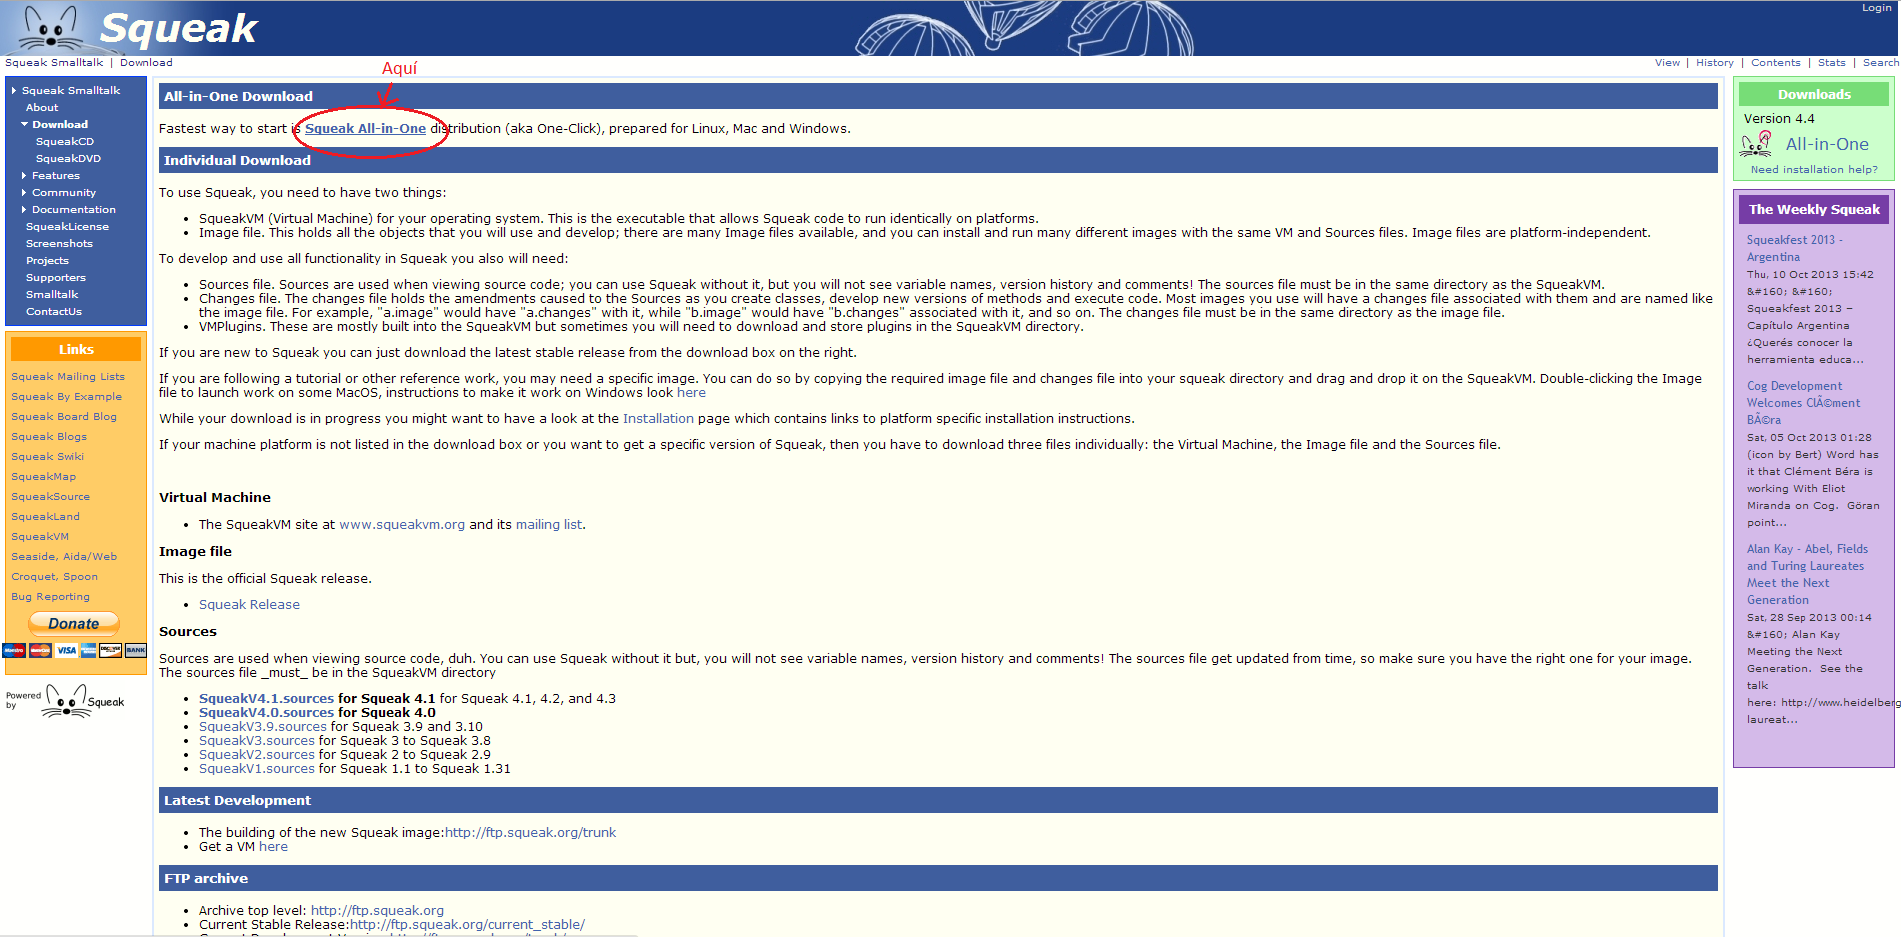
\includegraphics[width=0.8\textwidth]{images/tutorial}
				\end{center}
\paragraph{} \noindent
Una vez descargado lo descomprimimos en una carpeta y dentro encontraremos el ejecutable de Squeak para de aqui realizar nuestro primer programa en este lenguaje.

				\begin{center}
				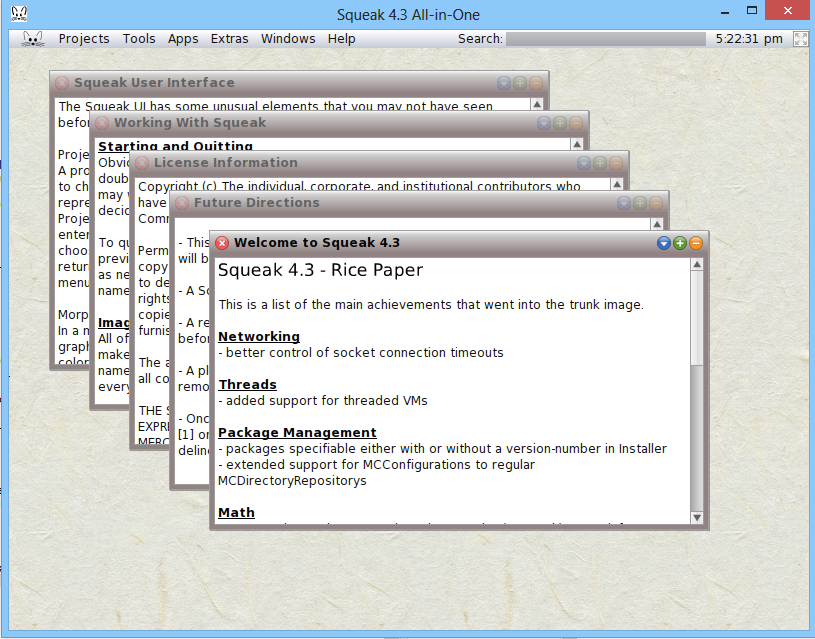
\includegraphics[width=0.8\textwidth]{images/squeak}
				\end{center}
\subsection{\textbf{Instalacion en Linux/Debian}}
\paragraph{} \noindent
Para instalar \textbf{Smalltalk} en sistemas Linux/Debian se debe primero agregar el repositorio que contiene el paquete Squeak, para hacerlo agregaremos las siguientes líneas al archivo  /etc/apt/source.list

\begin{lstlisting}
  deb http://ftp.squeak.org/debian/ stable main
  deb-src http://ftp.squeak.org/debian/ stable main
\end{lstlisting}
\paragraph{} \noindent
Este repositorio sólo esta disponible para sistemas Debian y sus derivados.
\paragraph{} \noindent
Una vez agregadas las líneas del repositorio que contiene squeak, abriremos el terminal y ejecutaremos los siguientes comandos
\begin{lstlisting}
$ sudo apt-get update
$ sudo apt-get install squeak squeak-plugin
\end{lstlisting}
\paragraph{} \noindent
Lo que actualizara la lista de repositorios e instalar Squeak, para ejecutar squeak debemos abrir la terminal y ejecutar
\begin{lstlisting}
$ squeak
\end{lstlisting}
\section{\textbf{Hola Mundo y otros Programas Introductorios}}
\subsection{\textbf{¡Hola Mundo!}}
\paragraph{}\noindent
Para comenzar a desarrollar en \textbf{Smalltalk} debemos hacer lo siguiente:
\begin{enumerate}
\item
En la barra de herramientas hacemos click en el menú `Projects'
				\begin{center}
				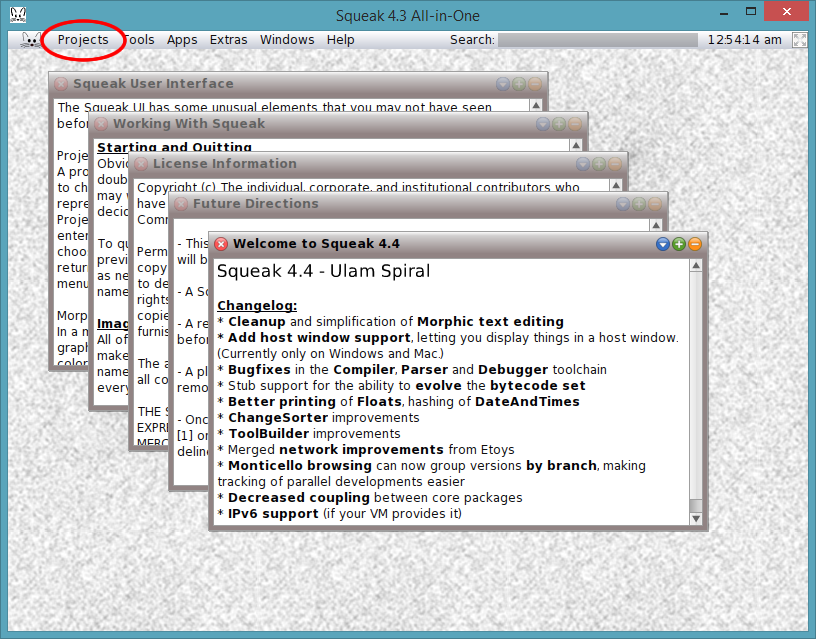
\includegraphics[width=0.5\textwidth]{images/barra_herramientas}
				\end{center}

\item
Elegimos la opcion `New Project', esta desplegará un submenú en el cual elegiremos la opción `New Morphic Project'
				\begin{center}
				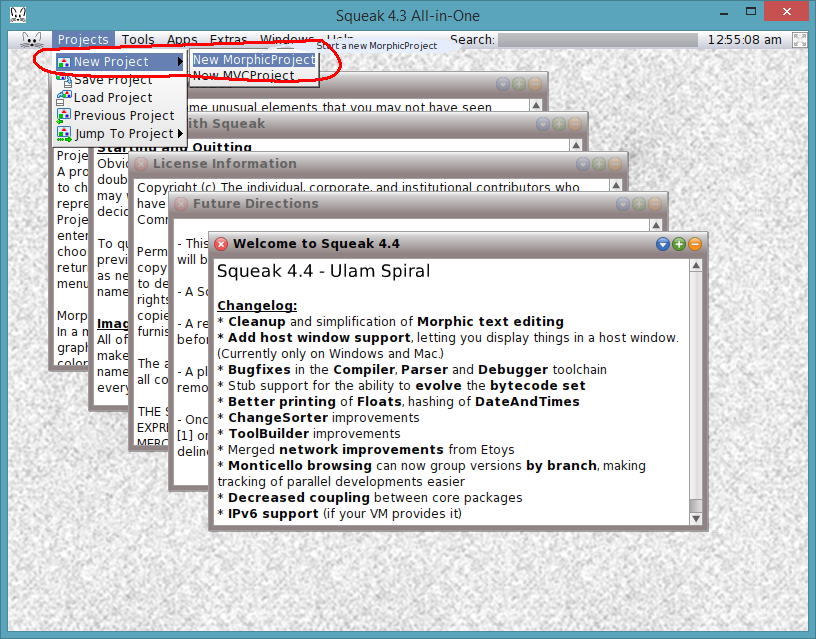
\includegraphics[width=0.5\textwidth]{images/new_project}
				\end{center}

\item
A continuación se desplegará una ventana con etiquetas, selecionaremos la etiqueta `Tools ' en el margen derecho de la ventana.
				\begin{center}
				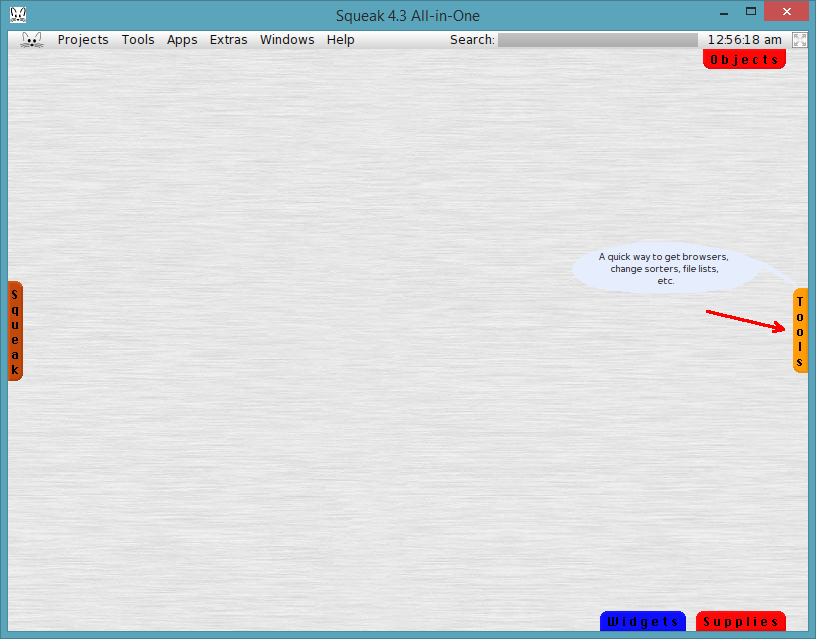
\includegraphics[width=0.5\textwidth]{images/tools}
				\end{center}
\item
Esto hará que se despliegue una barra lateral en la cual aparecen varias ventanas, arrastraremos las ventanas `Transcript' y `Workspace' en la parte principla de la ventana.
				\begin{center}
				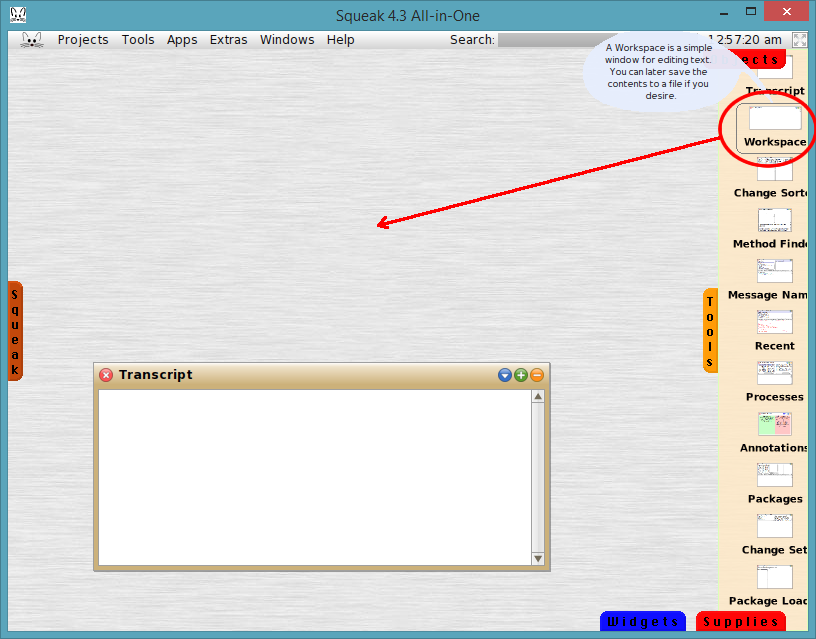
\includegraphics[width=0.5\textwidth]{images/drag_tools}
				\end{center}
\item
En la subventana `Workspace' escribiremos nuestro primer programa ``¡Hola Mundo!" del siguiente modo:
\begin{lstlisting}
Transcript show:`'Hola Mundo! 
\end{lstlisting}
ejecutamos con ctrl - D. En la subeventana `Transcript' podremos visualizar la ejecución de nuestro programa.
				\begin{center}
				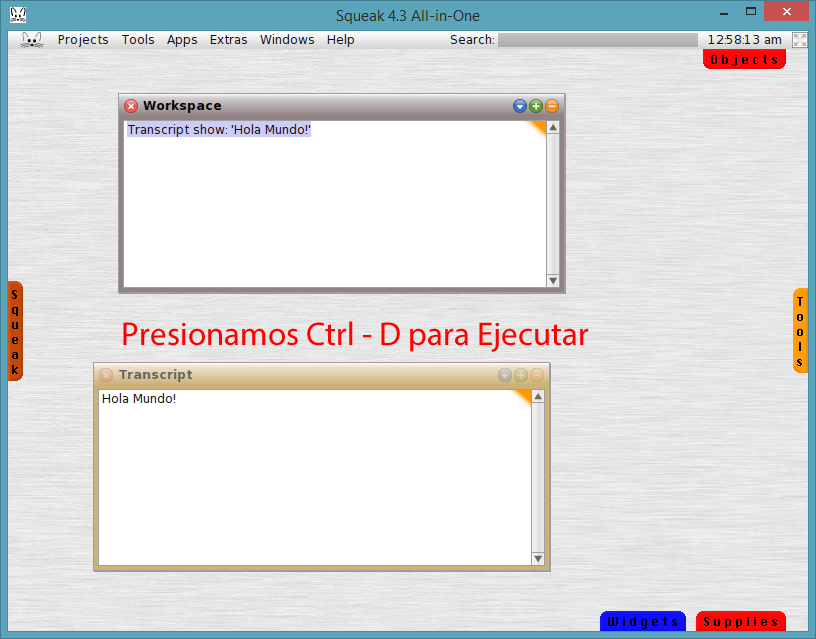
\includegraphics[width=0.5\textwidth]{images/executing}
				\end{center}

\subsection{\textbf{Suma de dos numeros}}
\paragraph{}\noindent
Para este ejemplo debemos seguir los pasos 1 - 4  del ejemplo anterior y en el `Workspace' escribimos:
\begin{lstlisting}
|var1 var2  var3| ``declaramos variables locales"
var1 := 2		  ``asignamos valores a variable 1"
var2 := 3		  ``asignamos valores a variable 2"
var3 := var1+var2 ``guardamos la suma de los 2 numeros en var3"
``Mostramos los valores y su resultado"
Transcript show: `Primer valor: ',var1,`  ',`Segundo valor: ',var2,`  ', `Resultado: ',var3 
\end{lstlisting}
\paragraph{}\noindent
Presionamos ctrl - D el resultado lo veremos en la venta `Transcript'.

				\begin{center}
				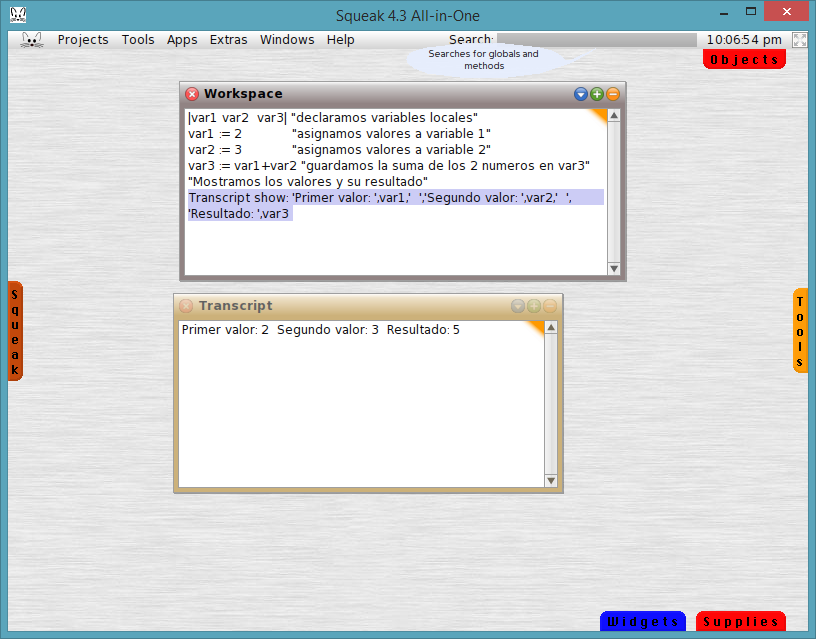
\includegraphics[width=0.5\textwidth]{images/second_example}
				\end{center}


\end{enumerate}



\section{Referencias}

\begin{enumerate}
	\item \href{http://computacion.cs.cinvestav.mx/~acaceres/courses/itesm/lp/clases/lp12.pdf}{http://computacion.cs.cinvestav.mx/~acaceres/courses/itesm/lp/clases/lp12.pdf}
\end{enumerate}


\bibliography{referencias}

\end{document}

